%%%%%%%%%%%%%%%%%%%%%%%%%%%%% Define Article %%%%%%%%%%%%%%%%%%%%%%%%%%%%%%%%%%
\documentclass{article}
%%%%%%%%%%%%%%%%%%%%%%%%%%%%%%%%%%%%%%%%%%%%%%%%%%%%%%%%%%%%%%%%%%%%%%%%%%%%%%%

%%%%%%%%%%%%%%%%%%%%%%%%%%%%% Using Packages %%%%%%%%%%%%%%%%%%%%%%%%%%%%%%%%%%
\usepackage{graphicx}
\usepackage[margin=0.8in]{geometry}
\usepackage{amssymb}
\usepackage{amsmath}
\usepackage{amsthm}
\usepackage{empheq}
\usepackage{rotating} % Include this package to use sidewaysfigure
\usepackage{mdframed}
\usepackage{booktabs}
\usepackage{float} % for the H specifier
\usepackage{placeins} % for \FloatBarrier
\usepackage{indentfirst}
\usepackage{lipsum}
\usepackage{graphicx}
\usepackage{booktabs} 
\usepackage{color}
\usepackage{psfrag}
\usepackage{pgfplots}
\usepackage{bm}
\usepackage{listings}
\usepackage{xcolor}
%%%%%%%%%%%%%%%%%%%%%%%%%%%%%%%%%%%%%%%%%%%%%%%%%%%%%%%%%%%%%%%%%%%%%%%%%%%%%%%

% Other Settings

%%%%%%%%%%%%%%%%%%%%%%%%%% Page Setting %%%%%%%%%%%%%%%%%%%%%%%%%%%%%%%%%%%%%%%
\geometry{a4paper}

%%%%%%%%%%%%%%%%%%%%%%%%%% Define some useful colors %%%%%%%%%%%%%%%%%%%%%%%%%%
\definecolor{ocre}{RGB}{243,102,25}
\definecolor{mygray}{RGB}{243,243,244}
\definecolor{deepGreen}{RGB}{26,111,0}
\definecolor{shallowGreen}{RGB}{235,255,255}
\definecolor{deepBlue}{RGB}{61,124,222}
\definecolor{shallowBlue}{RGB}{235,249,255}
%%%%%%%%%%%%%%%%%%%%%%%%%%%%%%%%%%%%%%%%%%%%%%%%%%%%%%%%%%%%%%%%%%%%%%%%%%%%%%%
\definecolor{codegreen}{rgb}{0,0.6,0}
\definecolor{codegray}{rgb}{0.5,0.5,0.5}
\definecolor{codepurple}{rgb}{0.58,0,0.82}
\definecolor{backcolour}{rgb}{0.95,0.95,0.92}

\lstdefinestyle{mystyle}{
    backgroundcolor=\color{backcolour},   
    commentstyle=\color{codegreen},
    keywordstyle=\color{magenta},
    numberstyle=\tiny\color{codegray},
    stringstyle=\color{codepurple},
    basicstyle=\ttfamily\footnotesize,
    breakatwhitespace=false,         
    breaklines=true,                 
    captionpos=b,                    
    keepspaces=true,                 
    numbers=left,                    
    numbersep=5pt,                  
    showspaces=false,                
    showstringspaces=false,
    showtabs=false,                  
    tabsize=2
}

\lstset{style=mystyle}
%%%%%%%%%%%%%%%%%%%%%%%%%% Define an orangebox command %%%%%%%%%%%%%%%%%%%%%%%%
\newcommand\orangebox[1]{\fcolorbox{ocre}{mygray}{\hspace{1em}#1\hspace{1em}}}
%%%%%%%%%%%%%%%%%%%%%%%%%%%%%%%%%%%%%%%%%%%%%%%%%%%%%%%%%%%%%%%%%%%%%%%%%%%%%%%

%%%%%%%%%%%%%%%%%%%%%%%%%%%% English Environments %%%%%%%%%%%%%%%%%%%%%%%%%%%%%
\newtheoremstyle{mytheoremstyle}{3pt}{3pt}{\normalfont}{0cm}{\rmfamily\bfseries}{}{1em}{{\color{black}\thmname{#1}~\thmnumber{#2}}\thmnote{\,--\,#3}}
\newtheoremstyle{myproblemstyle}{3pt}{3pt}{\normalfont}{0cm}{\rmfamily\bfseries}{}{1em}{{\color{black}\thmname{#1}~\thmnumber{#2}}\thmnote{\,--\,#3}}
\theoremstyle{mytheoremstyle}
\newmdtheoremenv[linewidth=1pt,backgroundcolor=shallowGreen,linecolor=deepGreen,leftmargin=0pt,innerleftmargin=20pt,innerrightmargin=20pt,]{theorem}{Theorem}[section]
\theoremstyle{mytheoremstyle}
\newmdtheoremenv[linewidth=1pt,backgroundcolor=shallowBlue,linecolor=deepBlue,leftmargin=0pt,innerleftmargin=20pt,innerrightmargin=20pt,]{definition}{Definition}[section]
\theoremstyle{myproblemstyle}
\newmdtheoremenv[linecolor=black,leftmargin=0pt,innerleftmargin=10pt,innerrightmargin=10pt,]{problem}{Problem}[section]
%%%%%%%%%%%%%%%%%%%%%%%%%%%%%%%%%%%%%%%%%%%%%%%%%%%%%%%%%%%%%%%%%%%%%%%%%%%%%%%

%%%%%%%%%%%%%%%%%%%%%%%%%%%%%%% Plotting Settings %%%%%%%%%%%%%%%%%%%%%%%%%%%%%
\usepgfplotslibrary{colorbrewer}
\pgfplotsset{width=8cm,compat=1.9}
%%%%%%%%%%%%%%%%%%%%%%%%%%%%%%%%%%%%%%%%%%%%%%%%%%%%%%%%%%%%%%%%%%%%%%%%%%%%%%%

%%%%%%%%%%%%%%%%%%%%%%%%%%%%%%% Title & Author %%%%%%%%%%%%%%%%%%%%%%%%%%%%%%%%
\title{\textbf{BANA 620 PROJECT REPORT: DESCRIPTIVE AND PREDICTIVE ANALYTICS APPLIED TO THE SKILLED NURSING FACILITY COST REPORTS}}
\author{Joshua Cabal \\ \\ \\California State University, Northridge \\}
%%%%%%%%%%%%%%%%%%%%%%%%%%%%%%%%%%%%%%%%%%%%%%%%%%%%%%%%%%%%%%%%%%%%%%%%%%%%%%%

\begin{document}
    \maketitle
    \pagebreak
    \tableofcontents    
    \newpage


%-------------------BEGIN: Executive Summary------------------------------------
\section{Executive Summary}

An overview of the project, including key findings, recommendations, and a brief summary of the analysis conducted. This section should be concise and geared toward readers who may not delve into the full details of the report. 

%-------------------END: Executive Summary------------------------------------
%-------------------BEGIN: Introduction------------------------------------
\section{Introduction}

Context and background information about the opportunity the project addresses. This section should outline the objectives of the project and the significance of the analysis being conducted.

\subsection{Context and Background Information}

Due to the significant number of baby boomers exploring nursing home options, your company has been tasked with determining whether it is advisable to suggest your client invest in nursing homes. As a member of the data analysis team, you are required to perform an analysis to address this question. Your team has acquired a comprehensive dataset of U.S. nursing homes for the years 2015-2021. 


\subsection{Objectives}

This study is guided by a series of specific objectives designed to deepen the understanding of the financial dynamics within the U.S. nursing home sector over the selected period. These objectives are outlined as follows:

\begin{enumerate}
    \item \textbf{Evaluate} the overall financial performance of nursing homes in the United States during this period.
    \item \textbf{Identify} the influential factors that affect the financial performance of these facilities.
    \item \textbf{Determine} the most significant factors that impact the performance of nursing homes, with a special emphasis on distinguishing between operational and external influences.
    \item \textbf{Describe} the trends observed in the performance of nursing homes and the dynamics of these influential factors over time.
    \item \textbf{Analyze} the specific impact of the COVID-19 pandemic on the financial and operational stability of nursing homes.
\end{enumerate}

In support of these objectives, the project will incorporate a comprehensive exploratory data analysis (EDA) to extract key insights from historical data spanning several years. Additionally, predictive analytics techniques will be employed to ascertain the most critical features influencing the sector’s performance. This analysis aims to provide actionable insights and data-driven recommendations to stakeholders considering investments in this industry.


%-------------------END: Introduction------------------------------------
%-------------------BEGIN: Methodology------------------------------------
\section{Methodology}

A detailed description of the analytical methods and tools used in the project. This should include data collection processes, data analysis techniques (e.g., statistical methods, machine learning algorithms), and any software or programming languages utilized.

\subsection{Software}
The entire analysis was conducted using Python (3.11.4) within the Jupyter Notebooks environment. The following Python libraries were used in the project:
\begin{enumerate}
    \item \textbf{Pandas} for data manipulation and cleaning.
    \item \textbf{NumPy} for numerical operations.
    \item \textbf{Scikit-learn} for implementing machine learning algorithms and preprocessing methods.
    \item \textbf{Matplotlib} and \textbf{Seaborn} for data visualization, facilitating the interpretation of results and comparison of model performance.
\end{enumerate}

These tools were selected for their robust functionality and widespread adoption in the data science community, enabling efficient data processing and modeling capabilities.

\subsection{Preprocessing Scalers}
Two different numerical scalers were used and compared. Below is the description of each method. 
\begin{enumerate}
    \item \textbf{Standard Scaler: } Standardize features by removing the mean and scaling to unit variance. The standard score of a sample x is calculated as:
    
    \[z = \frac{x-u}{s}\]
    
Centering and scaling happen independently on each feature by computing the relevant statistics on the samples in the training set. Mean and standard deviation are then stored to be used on later data using transform.

Standardization of a dataset is a common requirement for many machine learning estimators: they might behave badly if the individual features do not more or less look like standard normally distributed data (e.g. Gaussian with 0 mean and unit variance).

For instance many elements used in the objective function of a learning algorithm (such as the RBF kernel of Support Vector Machines or the L1 and L2 regularizers of linear models) assume that all features are centered around 0 and have variance in the same order. If a feature has a variance that is orders of magnitude larger than others, it might dominate the objective function and make the estimator unable to learn from other features correctly as expected.

    \item \textbf{Robust Scaler: } Scales features using statistics that are robust to outliers.

    This Scaler removes the median and scales the data according to the quantile range (defaults to IQR: Interquartile Range). The IQR is the range between the 1st quartile (25th quantile) and the 3rd quartile (75th quantile).
    
    Centering and scaling happen independently on each feature by computing the relevant statistics on the samples in the training set. Median and interquartile range are then stored to be used on later data using the transform method.
    
    Standardization of a dataset is a common preprocessing for many machine learning estimators. Typically this is done by removing the mean and scaling to unit variance. However, outliers can often influence the sample mean / variance in a negative way. In such cases, using the median and the interquartile range often give better results.
\end{enumerate}


\subsection{Machine Learning Models}
Severl different models were used and compared in this study to determine model suitability. Below are the details related to each method. 
\begin{enumerate}
    \item \textbf{Linear Regression}: Ordinary least squares Linear Regression. LinearRegression fits a linear model with coefficients w = (w1, …, wp) to minimize the residual sum of squares between the observed targets in the dataset, and the targets predicted by the linear approximation.
    \[
        \text{minimizes: } \, \frac{1}{2n} \sum_{i=1}^n \left(y_i - (\beta_0 + \beta_1 x_{i1} + \beta_2 x_{i2} + \dots + \beta_p x_{ip})\right)^2\]

where:
\begin{itemize}
    \item $n$ is the number of observations in the dataset.
    \item $y_i$ represents the observed value of the dependent variable for the $i$-th observation.
    \item $x_{ij}$ is the value of the $j$-th explanatory variable for the $i$-th observation.
    \item $\beta_j$ denotes the coefficient for the $j$-th explanatory variable, quantifying the effect of this variable on the response.
    \item $\beta_0$ is the intercept, representing the expected mean value of $y_i$ when all explanatory variables are equal to zero.
\end{itemize}


    \item \textbf{Lasso Regression}: Linear Model trained with L1 prior as regularizer (aka the Lasso). Regularization improves the conditioning of the problem and reduces the variance of the estimates. Larger values specify stronger regularization.
    \[
\text{minimizes: } \, \left\{ \frac{1}{2n} \sum_{i=1}^n (y_i - \mathbf{x}_i^\top \mathbf{\beta})^2 + \alpha \|\mathbf{\beta}\|_1 \right\}
\]

where:
\begin{itemize}
    \item $n$ represents the number of observations in the dataset.
    \item $y_i$ is the observed value of the dependent variable for the $i$-th observation.
    \item $\mathbf{x}_i$ is the vector of explanatory variables (features) for the $i$-th observation.
    \item $\mathbf{w}$ denotes the vector of coefficients (including the intercept and slopes) of the linear model.
    \item $\alpha$ is a non-negative regularization parameter that controls the strength of the L1 penalty, encouraging sparsity in the vector of coefficients.
    \item $\|\mathbf{w}\|_1$ represents the L1 norm of the coefficients, which is the sum of the absolute values of the coefficients.
\end{itemize}

    \item \textbf{Ridge Regression}: Linear least squares with L2 regularization. This model solves a regression model where the loss function is the linear least squares function and regularization is given by the l2-norm
       \[
        \text{minimizes: } \, \frac{1}{2n} \sum_{i=1}^n \left(y_i - (\beta_0 + \beta_1 x_{i1} + \beta_2 x_{i2} + \dots + \beta_p x_{ip})\right)^2 + \lambda \sum_{j=1}^p \beta_j^2\] 
        where:
\begin{itemize}
    \item $n$ is the number of observations in the dataset.
    \item $y_i$ represents the observed value of the dependent variable for the $i$-th observation.
    \item $x_{ij}$ is the value of the $j$-th explanatory variable for the $i$-th observation.
    \item $\beta_j$ denotes the coefficient for the $j$-th explanatory variable, quantifying the effect of this variable on the response.
    \item $\beta_0$ is the intercept, representing the expected mean value of $y_i$ when all explanatory variables are equal to zero.
    \item $\lambda$ is a non-negative regularization parameter that controls the strength of the penalty applied to the size of the coefficients.
\end{itemize}

    
    \item \textbf{Elastic Net}: Linear regression with combined L1 and L2 priors as regularizer.
    \[
        \text{minimizes: } \, \frac{1}{2n} \sum_{i=1}^n \left(y_i - (\beta_0 + \beta_1 x_{i1} + \beta_2 x_{i2} + \dots + \beta_p x_{ip})\right)^2 + \lambda \left( \alpha \sum_{j=1}^p |\beta_j| + \frac{1-\alpha}{2} \sum_{j=1}^p \beta_j^2 \right)
\]
where:
\begin{itemize}
    \item $n$ is the number of observations in the dataset.
    \item $y_i$ represents the observed value of the dependent variable for the $i$-th observation.
    \item $x_{ij}$ is the value of the $j$-th explanatory variable for the $i$-th observation.
    \item $\beta_j$ denotes the coefficient for the $j$-th explanatory variable, quantifying the effect of this variable on the response.
    \item $\beta_0$ is the intercept, representing the expected mean value of $y_i$ when all explanatory variables are equal to zero.
    \item $\lambda$ is a non-negative regularization parameter that controls the overall strength of the penalty.
    \item $\alpha$ is a parameter between 0 and 1 that balances the contribution of L1 and L2 penalties: $\alpha$ for the L1 component and $(1-\alpha)$ for the L2 component.
\end{itemize}


    \item \textbf{K Neighbors Regressor}: Regression based on k-nearest neighbors. The target is predicted by local interpolation of the targets associated of the nearest neighbors in the training set.
        \[
\text{prediction for } x_q = \frac{1}{K} \sum_{i \in N_K(x_q)} y_i
\]
\begin{itemize}
    \item $x_q$ is the query point for which the prediction is to be made.
    \item $K$ is the number of nearest neighbors considered for making the prediction.
    \item $N_K(x_q)$ is the set of indices of the $K$ nearest neighbors to $x_q$.
    \item $y_i$ are the observed values of the dependent variable for the neighbors.
\end{itemize}
\end{enumerate}



%-------------------END: Methodology------------------------------------
%-------------------BEGIN: Data Description------------------------------------
\section{Data Description}

An overview of the data set(s) used, including sources, size, and characteristics of the data. Highlight any data cleaning or preprocessing steps undertaken to prepare the data for analysis.



\subsection{Skilled Nusing Facility Cost Report}

Medicare-certified institutional providers are required to submit annual cost reports. These data files contain the highest level of cost report status for cost reports in each reported fiscal years. The cost report contains provider information such as facility characteristics, utilization data, cost and charges by cost center (in total and for Medicare), Medicare settlement data, and financial statement data. CMS maintains the cost report data in the Healthcare Provider Cost Reporting Information System (HCRIS). Skilled Nursing Facilities (SNF) submit their cost report data to HCRIS using form CMS-2540-2010. The reports used are from the years 2015 through 2021.

\subsubsection{Data Loading and Handling Missing Values}

Each file comprises annual cost reports for over 15,000 skilled nursing facilities, all stored in separate CSV files for each of the years under study. To facilitate analysis, these files required concatenation into a single DataFrame. Initially, inconsistencies in column headers across the files for the years 2020 and 2021 were modified to match with those of previous years. This matching was manually executed in Microsoft Excel by renaming similar columns accordingly and discarding unmatched columns. Additionally, a \texttt{Year} attribute was appended to each record during the import step to preserve the, and all column headers were converted to lowercase to ensure consistency.

Following the import, the primary focus shifted to managing null values within the dataset. The initial step involved column-level cleaning, where I established two distinct lists of columns slated for removal: \texttt{dropNull} and \texttt{dropRedundancy}. The \texttt{dropNull} list encompassed columns that exhibited excessive nullity, with more than 90\% of their values missing across all records. The \texttt{dropRedundancy} list comprised columns that provided redundant information, which was otherwise encapsulated by other attributes. Given that the financial forms required a detailed breakdown of reported figures, only the most aggregated data were retained by removing the redundant columns.

To address the remaining null values, record-level cleaning was conducted through simple imputation. Specifically, mean imputation was employed, and the imputed values were rounded to the nearest integer. This rounding was justified as several of the attributes inherently attain only integer values. After these preprocessing steps, the dataset was streamlined from an initial 100 columns to 55, thereby enhancing the manageability and potential predictive accuracy of the ensuing models.

\subsubsection{Handling Outliers}
The initial approach to managing outliers involved the application of a z-score threshold method. This technique operates by setting a specific z-score limit and excluding all records that exhibit values beyond this predefined range. For this analysis, a threshold of 3 was selected, focusing specifically on the variables 'net income' and 'accounts payable.' This decision was informed by extensive testing across various attributes and different threshold settings, which demonstrated that targeting these particular columns effectively addressed a significant portion of the outliers.

\begin{lstlisting}[language=Python, caption=Function to clean by z-score threshold]
# dealing with a subset of outliers by z-score threshold
def removeOutliers(input_df, column_name, zScoreThreshold):
    mean = input_df[column_name].mean()
    std = input_df[column_name].std()
    z_scores = (input_df[column_name] - mean) / std

    return input_df[(z_scores > -zScoreThreshold) & (z_scores < zScoreThreshold)]

numerical_columns = ['net_income', 'accounts_payable']
for each in numerical_columns:
   df = removeOutliers(fullCostReportdf, each, 3)
\end{lstlisting}

Upon completion of the initial outlier management, a subsequent manual review of the dataset was conducted to identify any additional outliers. This examination revealed that the attribute \texttt{number of beds} contained suspect outliers. Specifically, eleven nursing facilities reported possessing in excess of 21,000 beds. To address this anomaly, a variable named bedThreshold was defined and set at 21,000. All records exceeding this threshold were subsequently removed from the dataset to ensure the integrity and accuracy of the analysis.

\subsubsection{Feature Engineering}
This study employs feature engineering techniques to derive additional predictive insights from the dataset's financial metrics. Recognizing that interactions among variables can potentially encapsulate a greater degree of variance than the individual variables in isolation, we have constructed additional features which aim to capture information related to the financial health of the nursing homes. These newly defined features, which capitalize on the interactions between existing variables, are posited to possibly enhance the predictive capacity of the resultant model. Specifically, the following features were engineered and incorporated into the analysis:

\begin{enumerate}
    \item \textbf{Profit Margins:}
    \begin{itemize}
        \item Gross Profit Margin: (\textbf{\texttt{gross\_revenue}} - \textbf{\texttt{total\_costs}}) / \textbf{\texttt{gross\_revenue}}.
        \item Net Profit Margin: \textbf{\texttt{net\_income}} / \textbf{\texttt{gross\_revenue}}.
    \end{itemize}
    
    \item \textbf{Operational Efficiency:}
    \begin{itemize}
        \item Total Operating Expense Ratio: \textbf{\texttt{less\_total\_operating\_expense}} / \textbf{\texttt{gross\_revenue}}.
    \end{itemize}
    
    \item \textbf{Liquidity Ratios:}
    \begin{itemize}
        \item Current Ratio: \textbf{\texttt{total\_current\_assets}} / \textbf{\texttt{total\_current\_liabilities}}.
    \end{itemize}
    
    \item \textbf{Solvency Ratios:}
    \begin{itemize}
        \item Debt-to-Equity Ratio: \textbf{\texttt{total\_liabilities}} / \textbf{\texttt{total\_fund\_balances}}.
    \end{itemize}
    
    \item \textbf{Return on Investment (ROI):}
    \begin{itemize}
        \item ROI: \textbf{\texttt{net\_income}} / \textbf{\texttt{total\_assets}}.
    \end{itemize}
    
    \item \textbf{Capacity Utilization:}
    \begin{itemize}
        \item Bed Occupancy Rate: \textbf{\texttt{total\_days\_total}} / (\textbf{\texttt{number\_of\_beds}} $\times$ 365).
    \end{itemize}
    
    \item \textbf{Cost Management:}
    \begin{itemize}
        \item Cost per Bed: \textbf{\texttt{total\_costs}} / \textbf{\texttt{number\_of\_beds}}.
        \item Salary Costs per Bed: \textbf{\texttt{total\_salaries\_adjusted}} / \textbf{\texttt{number\_of\_beds}}.
    \end{itemize}
\end{enumerate}

In subsequent analyses, not all of the aforementioned features demonstrated statistical significance. This observation is elaborated upon in the later sections of this study, where the impact of each variable on the model's performance is evaluated.

\subsubsection{Feature Scaling and Encoding}
The preprocessing stage of the analysis involved the application of two normalization techniques to prepare the dataset for subsequent modeling: \texttt{StandardScaler()} and \texttt{RobustScaler()}. These scaling methods were selected to assess the data’s behavior under different normalization conditions and to mitigate the influence of outliers that could skew the results of more sensitive algorithms. The results of these methods will be detailed below in the Analysis section. 

Categorical variables were transformed through one-hot encoding to facilitate their integration into the regression models. This process was executed using the \texttt{pd.get\_dummies()} function from the Pandas library. The specific features subjected to this encoding method were \texttt{state\_code} and \texttt{rural\_versus\_urban}, enabling the models to handle these categorical inputs effectively.


\subsection{Provider Information}
General information on currently active nursing homes, including number of certified beds, quality measure scores, staffing and other information used in the Five-Star Rating System

CMS created the Five-Star Quality Rating System to help consumers, their families, and caregivers compare nursing homes more easily and to help identify areas about which you may want to ask questions.  The Nursing Home Care Compare web site features a quality rating system that gives each nursing home a rating of between 1 and 5 stars.  Nursing homes with 5 stars are considered to have much above average quality and nursing homes with 1 star are considered to have quality much below average.  There is one Overall 5-star rating for each nursing home, and separate ratings for health inspections, staffing and quality measures.

\subsection{Exporatory Data Analysis}

\subsection{Exporatory Data Analysis}
hello world!

%-------------------BEGIN: Analysis and Findings------------------------------------
\section{Analysis and Findings}

Presentation of the analysis conducted, including data visualization (charts, graphs, tables) and statistical outputs. This section should detail the insights gained from the analysis, interpreting the results in the context of the business problem.


\subsection{Model Fit and Comparison for Cost Report Dataset}
The analysis incorporated two distinct normalization techniques: \texttt{StandardScaler()} and \texttt{RobustScaler()}. These scalers were selected to evaluate the robustness and performance of the models under different scaling conditions. The regression algorithms employed in the study included Linear Regression, Lasso Regression, Ridge Regression, Elastic Net Regression, and K-Nearest Neighbors Regression. Each model was systematically applied to the dataset after the application of each scaler to determine the impact on the predictive accuracy. The implementation of these models is detailed below:

\begin{lstlisting}[language=Python, caption=Regression model pipeline code]
def evaluate_regression_models(df, target_column, scaler, test_size=0.1, random_state=123):
    """
    Evaluate various regression models on a given DataFrame with specified scaler.

    Parameters:
    - df : DataFrame containing the data.
    - target_column : string, the name of the column to predict.
    - scaler : Scaler object from sklearn.preprocessing.
    - test_size : float, the proportion of the dataset to include in the test split.
    - random_state : int, random_state is the seed used by the random number generator.
    """
    
    X = df.drop([target_column], axis=1)
    y = df[target_column]

    # Define numerical features for scaling
    numericalFeatures = X.columns[X.dtypes != 'object']

    # Preprocessor using ColumnTransformer to apply scaling only to numerical features
    preprocessor = ColumnTransformer(
        transformers=[
            ('num', scaler, numericalFeatures)
        ])

    models = {
        'Linear Regression': LinearRegression(),
        'Ridge': Ridge(alpha=20000),
        'Lasso': Lasso(alpha=20000),
        'ElasticNet': ElasticNet(alpha=1.0, l1_ratio=0.5),
        'KNN': KNeighborsRegressor(n_neighbors=2)
    }

    results = pd.DataFrame(index=models.keys(), columns=['Mean Squared Error', 'R-squared'])

    # Iterate over models, create a full pipeline, and evaluate
    for name, model in models.items():
        pipeline = Pipeline(steps=[('preprocessor', preprocessor),
                                   ('regressor', model)])
        # Split data into train and test sets
        X_train, X_test, y_train, y_test = train_test_split(X, y, test_size=test_size, random_state=random_state)
        # Fit the model
        pipeline.fit(X_train, y_train)
        # Predict
        y_pred = pipeline.predict(X_test)
        # Evaluate
        mse = mean_squared_error(y_test, y_pred)
        r2 = r2_score(y_test, y_pred)
        results.loc[name] = [mse, r2]

    print(results)

    # Plotting results
    fig, ax = plt.subplots(1, 2, figsize=(14, 6))
    results.plot(kind='bar', y='Mean Squared Error', ax=ax[0], color='skyblue', title=f'Mean Squared Error by Model (Scaler: {scaler})')
    results.plot(kind='bar', y='R-squared', ax=ax[1], color='orange', title=f'R-squared by Model (Scaler: {scaler})')
    plt.tight_layout()
    plt.show()
\end{lstlisting}

Given the above results, 

\pagebreak

The performance of various regression models on the dataset is summarized in the figures and tables below. The metrics used for evaluation are Mean Squared Error (MSE) and the coefficient of determination (R-squared).

\begin{figure}[htbp]
\centering
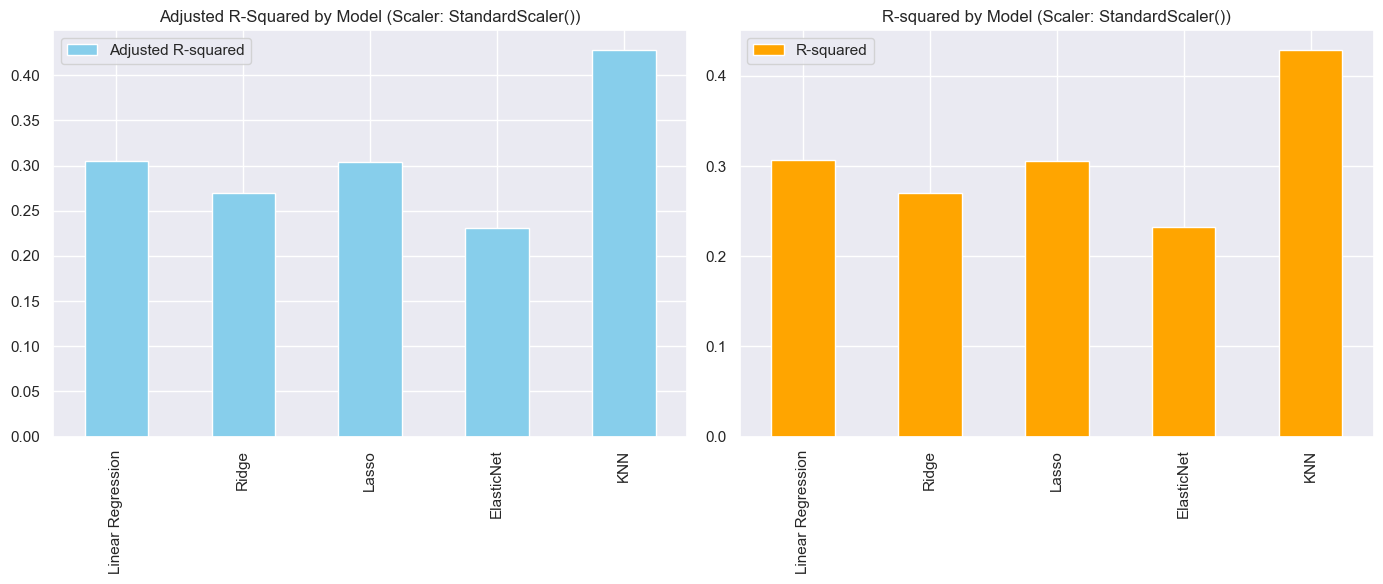
\includegraphics[width=\linewidth]{./Images/evalRegModelStandardScaler.png}
\caption{Results for \texttt{StandardScaler()}}
\label{fig:Standard Scaler Results}
\end{figure}

\begin{table}[ht]
\centering
\begin{tabular}{@{}lrr@{}}
\toprule
Model            & \multicolumn{1}{c}{Mean Squared Error} & \multicolumn{1}{c}{R-squared} \\ 
\midrule
Linear Regression & 3.97e12 & 0.416 \\
Ridge             & 3.09e12 & 0.545 \\
Lasso             & 2.78e12 & 0.591 \\
ElasticNet        & 3.50e12 & 0.485 \\
KNN               & 3.91e12 & 0.424 \\
\bottomrule
\end{tabular}
\label{tab:model_performance standard}
\end{table}

\FloatBarrier % Prevent floats from moving past this point
\pagebreak

\begin{figure}[htbp]
\centering
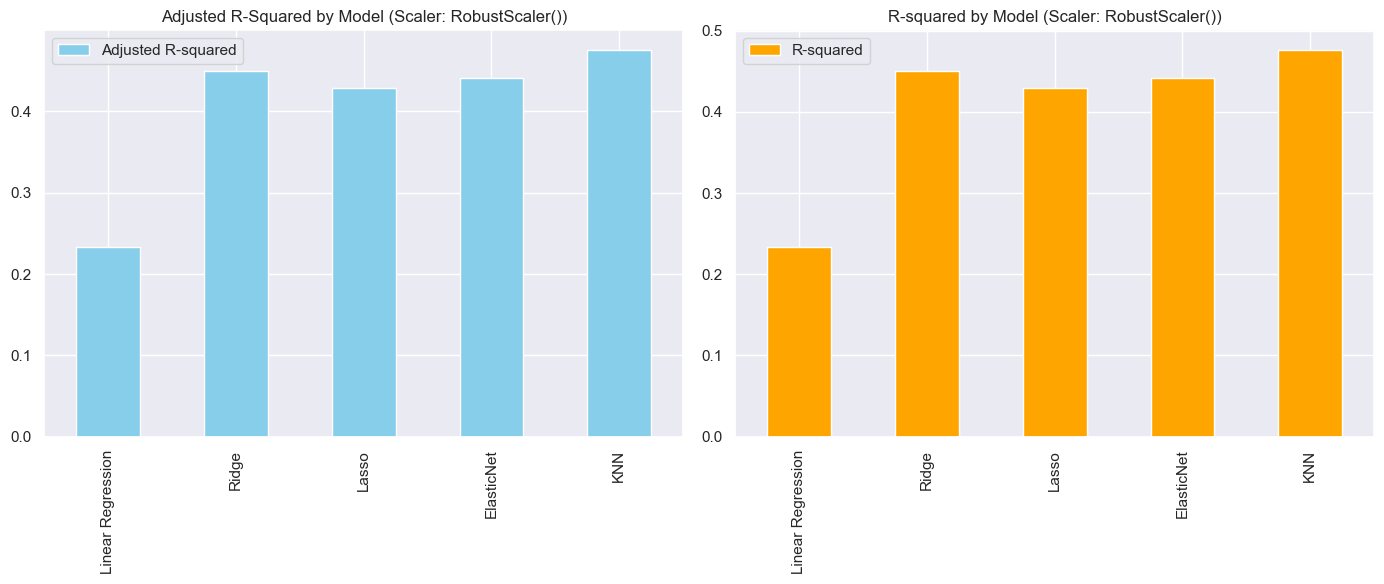
\includegraphics[width=\linewidth]{Images/evalRegModelRobustScaler.png}
\caption{Results for \texttt{RobustScaler()}}
\label{fig:Robust Scaler Results}
\end{figure}


\begin{table}[ht]
\centering
\begin{tabular}{@{}lrr@{}}
\toprule
Model            & \multicolumn{1}{c}{Mean Squared Error} & \multicolumn{1}{c}{R-squared} \\ 
\midrule
Linear Regression & 3.98e12 & 0.415 \\
Ridge             & 2.77e12 & 0.593 \\
Lasso             & 2.82e12 & 0.585 \\
ElasticNet        & 2.81e12 & 0.587 \\
KNN               & 2.90e12 & 0.574 \\
\bottomrule
\end{tabular}
\label{tab:model_performance robust}
\end{table}

\FloatBarrier % Another barrier to keep subsequent sections or floats in place

\pagebreak

\subsection{Regression Coefficients}

In quantitative analysis via Ridge regression, the magnitude and sign of the model's coefficients are indicative of the predictors' association with the target variable—net income of nursing homes. Higher absolute values denote stronger influence, with positive coefficients suggesting an increasing relationship, and negative ones indicating a decreasing effect. These interpretations, subject to the constraints of multicollinearity and the Ridge regularization, underscore associations rather than causality and are contingent upon the standardized scales of the predictors. This analysis aims to discern the contributory factors to net income while considering the implications of model constraints and the data's inherent characteristics.


\begin{figure}[htbp]
\centering
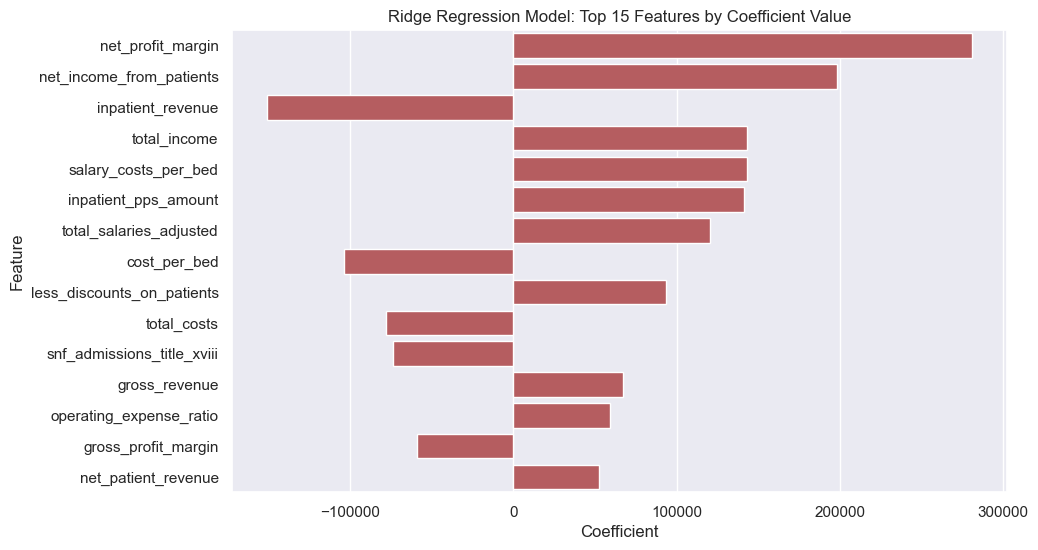
\includegraphics[width=\linewidth]{Images/feat_importance.png}
\caption{Ridge Regression: Top 15 Coefficient Values by Absolute Value}
\label{fig:Robust Scaler Results}
\end{figure}



\begin{table}[ht]
\centering
\begin{tabular}{@{}lrr@{}}
\toprule
{Feature} & {Coefficient} \\
\midrule
net\_profit\_margin & 280896 \\
net\_income\_from\_patients & 198654 \\
inpatient\_revenue & -151016 \\
total\_income & 143121 \\
salary\_costs\_per\_bed & 142947 \\
inpatient\_pps\_amount & 141518 \\
total\_salaries\_adjusted & 120431 \\
cost\_per\_bed & -103994 \\
less\_discounts\_on\_patients & 93425 \\
total\_costs & -78359 \\
snf\_admissions\_title\_xviii & -73877 \\
gross\_revenue & 67064 \\
operating\_expense\_ratio & 59231 \\
gross\_profit\_margin & -59231 \\
net\_patient\_revenue & 52355 \\
\bottomrule
\end{tabular}
\label{tab:model_performance robust}
\end{table}

\pagebreak



\begin{figure}[htbp]
\centering
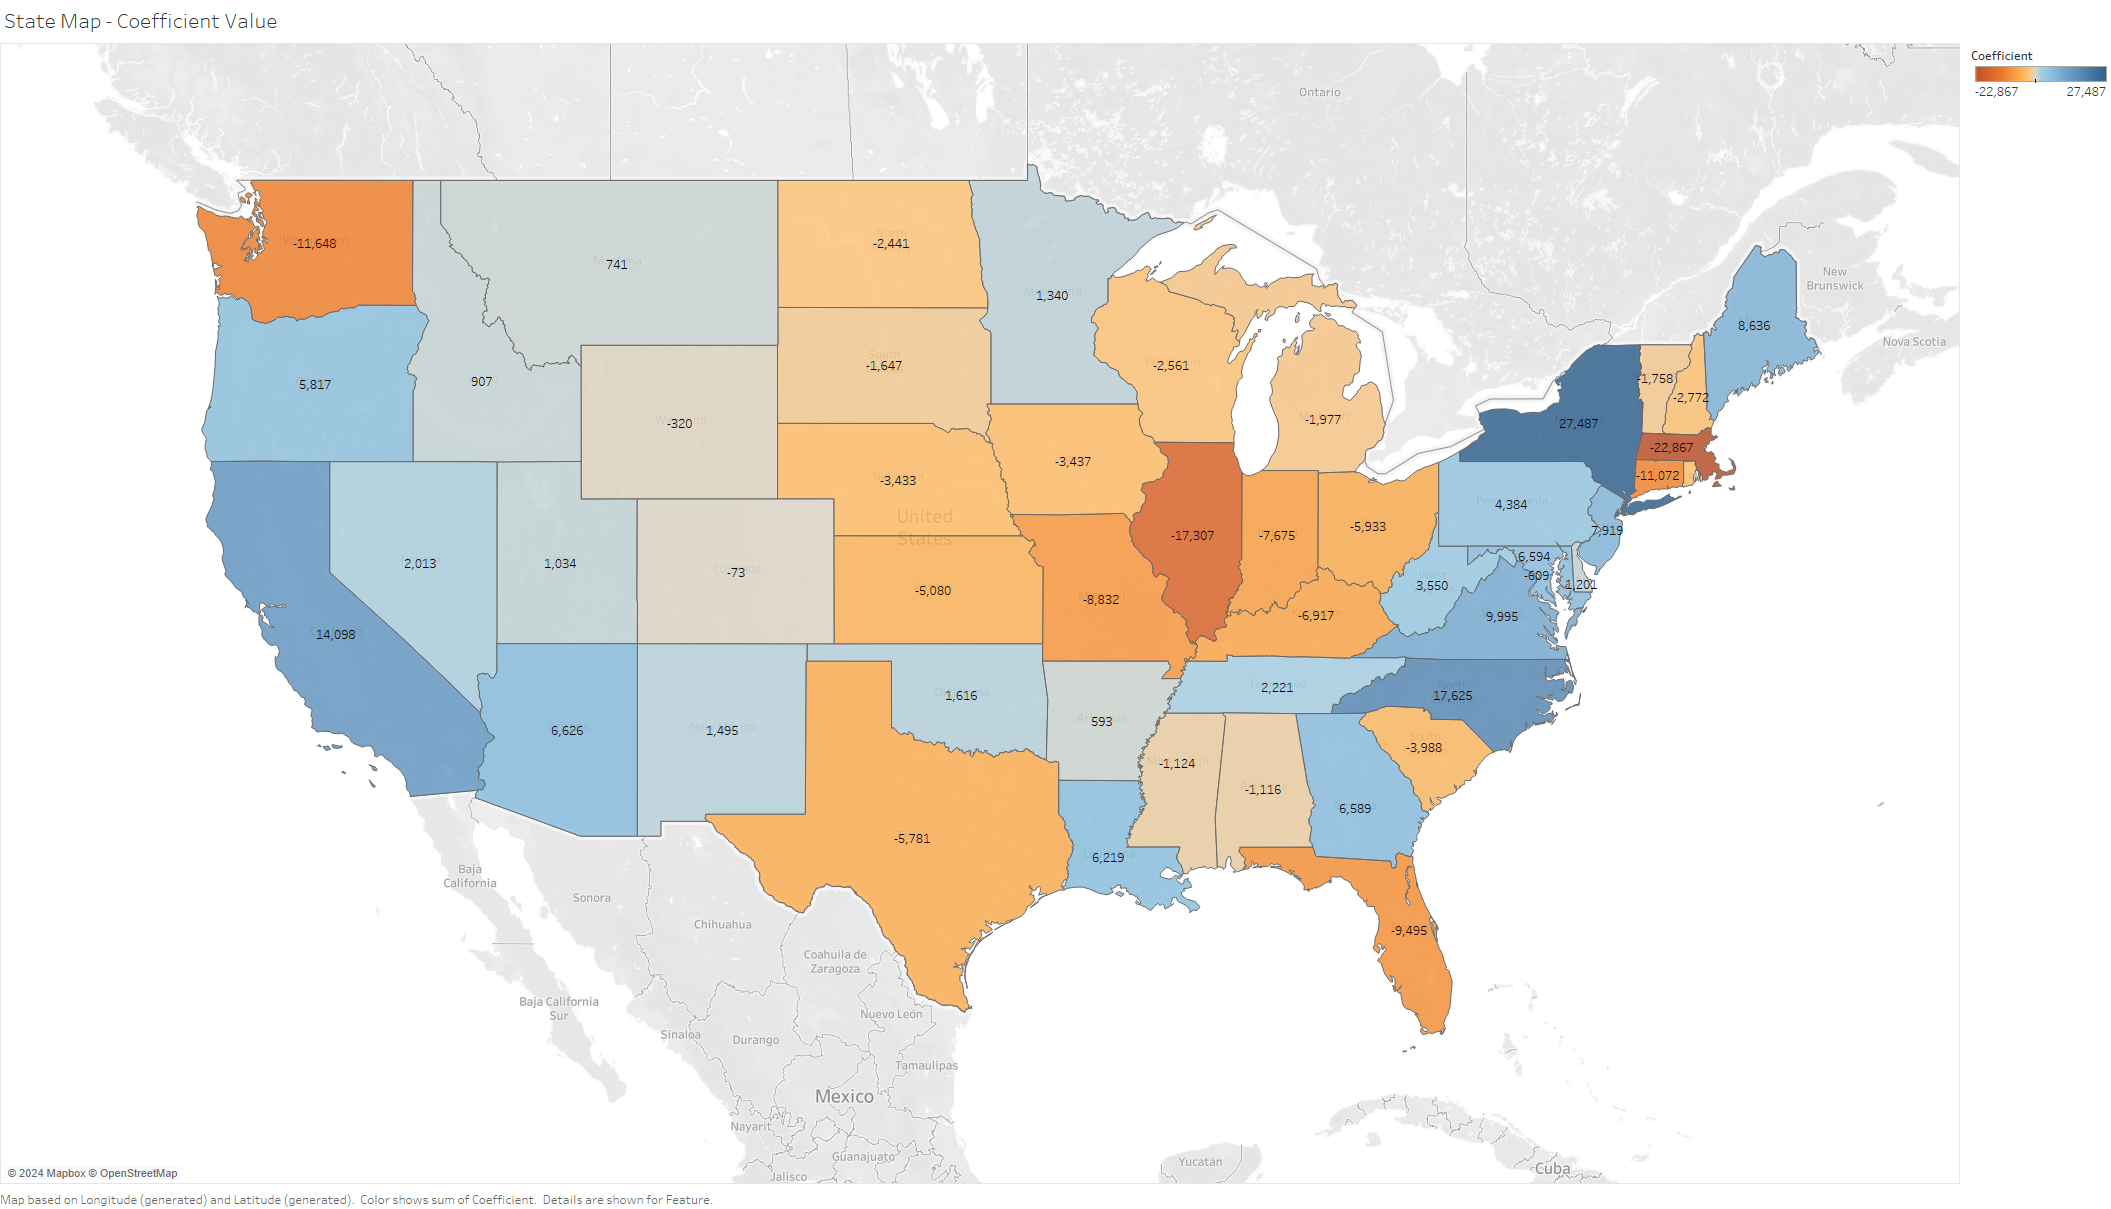
\includegraphics[width=\linewidth]{Images/State Map - Coefficient Value.png}
\caption{State Map - Ridge Regression Coefficients}
\label{fig:Robust Scaler Results}
\end{figure}

\begin{table}[htbp]
\centering
\label{tab:feature_importance}
\begin{tabular}{lc}
\toprule
Feature & {Coefficient} \\
\midrule
NY & 27486.53 \\
NC & 17624.84 \\
CA & 14097.99 \\
VA & 9995.25 \\
ME & 8635.73 \\
NJ & 7918.63 \\
AZ & 6626.17 \\
MD & 6593.83 \\
... & ... \\
KY & -6916.69 \\
IN & -7675.09 \\
MO & -8831.85 \\
FL & -9495.18 \\
CT & -11071.54 \\
WA & -11647.73 \\
IL & -17307.36 \\
MA & -22867.15 \\


\bottomrule
\end{tabular}
\end{table}

\pagebreak





%-------------------END: Analysis and Findings------------------------------------
%-------------------BEGIN: Discussion------------------------------------
\section{Discussion}
Interpretation of the findings, discussing how they address the project objectives and their implications for the business. This section should also cover any limitations of the analysis and considerations for future research.

%-------------------END: Discussion------------------------------------
%-------------------BEGIN: Recommendations------------------------------------
\section{Recommendations}
Based on the analysis and findings, provide actionable recommendations for the business. Clearly articulate the expected impact of these recommendations and suggest a plan for implementation.

%-------------------END: Recommendations------------------------------------
%-------------------BEGIN: Conclusion------------------------------------
\section{Conclusion}
Summarize the key points from the report, reinforcing the value of the findings and recommendations.

%-------------------END: Conclusion------------------------------------
%-------------------BEGIN: Appendices------------------------------------
\section{Appendices}
Include any additional material that supports the analysis, such as detailed data tables, code snippets, or extended methodology descriptions.

\begin{figure}[htbp]
\centering
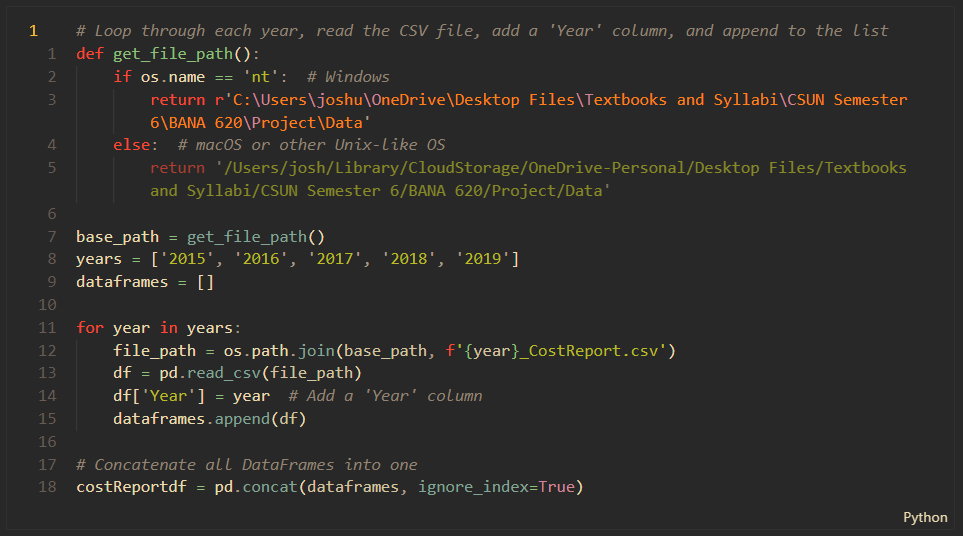
\includegraphics[width=\linewidth]{./Images/dataLoadingSnippet.png}
\caption{Data loading code snippet}
\label{fig:screenshot_label}
\end{figure}

%-------------------END: Appendices------------------------------------

%-------------------BEGIN: References------------------------------------
\section{References}
List all sources cited in the report, including data sources, literature, and any external references used in the analysis.

%-------------------END: References------------------------------------



\end{document}